\documentclass[aspectratio=169,11pt]{beamer}
\usetheme{default}
\usefonttheme{professionalfonts}
\usepackage[T1]{fontenc}
\usepackage{booktabs,amsmath,tikz}
\usetikzlibrary{shapes.geometric,arrows.meta,positioning,calc}

% ---- light background palette ----
\definecolor{bg}{HTML}{F7F9FC}
\definecolor{ink}{HTML}{1F2A44}
\definecolor{accent}{HTML}{2F6FDE}
\definecolor{accent2}{HTML}{E07A1F}
\definecolor{soft}{HTML}{E4ECF9}
\definecolor{good}{HTML}{2E8B57}
\definecolor{bad}{HTML}{C0392B}
\setbeamercolor{background canvas}{bg=bg}
\setbeamercolor{normal text}{fg=ink}
\setbeamercolor{structure}{fg=accent}
\setbeamercolor{frametitle}{fg=accent}
\setbeamercolor{title}{fg=accent}
\setbeamercolor{itemize item}{fg=accent}
\setbeamercolor{itemize subitem}{fg=accent2}
\setbeamertemplate{navigation symbols}{}
\setbeamertemplate{frametitle}{%
  \vskip1.2ex\usebeamerfont{frametitle}\usebeamercolor[fg]{frametitle}\insertframetitle\par
  \vskip0.6ex{\color{accent}\hrule height 1.2pt}}
\setbeamertemplate{footline}{%
  \hfill{\scriptsize\color{ink!60}\insertframenumber/\inserttotalframenumber}\hspace{1em}\vskip1ex}
\setbeamerfont{frametitle}{size=\Large,series=\bfseries}

\title{Sentence Style Detection for Author Switches}
\subtitle{Author Switch Detection}
\author{Tshephang Phuti-A-Nkutu Matlala}
\date{}

\begin{document}

\begin{frame}[plain]
\vspace{1.2cm}
{\usebeamercolor[fg]{title}\Huge\bfseries\inserttitle\par}
\vspace{0.4cm}
{\Large\color{ink!80}\insertsubtitle\par}
\vspace{0.8cm}
{\large\insertauthor}\\[0.3em]
{\color{ink!70}PAN 2026 Multi-Author Writing Style Analysis}
\end{frame}

\begin{frame}{Outline}
\begin{enumerate}
\setlength\itemsep{0.7em}
\item Representation \& features
\item Models overview
\item Results and interpretation
\item What I am still working on
\item Upcoming: estimating the number of authors
\end{enumerate}
\end{frame}

%% ---------------- (1) Representation & features ----------------
\begin{frame}{Task and data}
\textbf{Task:} for every pair of adjacent sentences $(S_i,S_{i+1})$, decide whether the author changes.
\medskip
\begin{columns}[T]
\begin{column}{0.5\textwidth}
\begin{itemize}
\item PAN 2026 data
\item Easy: topic changes with author. Medium/hard: topic is controlled
\item 2,439,074 training pairs, about 14.3\% of them are switches
\end{itemize}
\end{column}
\begin{column}{0.5\textwidth}
\centering\small
\begin{tabular}{lrr}
\toprule
& \textbf{Pairs} & \textbf{Switch rate}\\
\midrule
Easy & 549,804 & 30.5\%\\
Medium & 1,299,324 & 4.4\%\\
Hard & 589,946 & 20.9\%\\
\bottomrule
\end{tabular}
\end{column}
\end{columns}
\medskip
\begin{block}{}
Switch rates differ sharply by difficulty (easy, medium and hard).
\end{block}
\end{frame}

\begin{frame}{Pipeline: from raw text to a prediction}
\centering
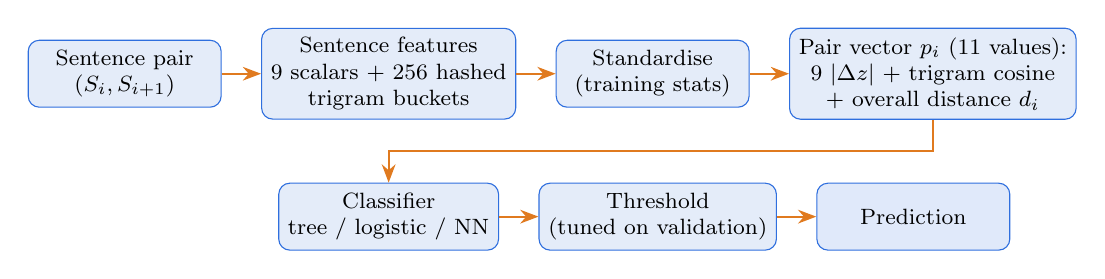
\begin{tikzpicture}[
  box/.style={draw=accent,fill=soft,rounded corners=4pt,minimum height=0.85cm,minimum width=2.45cm,align=center,font=\footnotesize},
  arr/.style={-{Stealth},thick,color=accent2}, node distance=0.5cm]
\node[box] (a) {Sentence pair\\$(S_i,S_{i+1})$};
\node[box,right=of a] (b) {Sentence features\\9 scalars + 256 hashed\\trigram buckets};
\node[box,right=of b] (c) {Standardise\\(training stats)};
\node[box,right=of c] (d) {Pair vector $p_i$ (11 values):\\9 $|\Delta z|$ + trigram cosine\\+ overall distance $d_i$};
\node[box,below=0.8cm of b] (e) {Classifier\\tree / logistic / NN};
\node[box,right=of e] (f) {Threshold\\(tuned on validation)};
\node[box,right=of f,fill=accent!15] (g) {Prediction};
\draw[arr] (a)--(b); \draw[arr] (b)--(c); \draw[arr] (c)--(d);
\draw[arr] (d.south) -- ++(0,-0.4) -| ($(e.north)+(0,0.0)$) ;
\draw[arr] (e)--(f); \draw[arr] (f)--(g);
\end{tikzpicture}
\medskip

\begin{itemize}\itemsep0.3em
\item Written in Java with \emph{no external ML library}.
\end{itemize}
\end{frame}

\begin{frame}{Nine style features used during training}
\centering\small
\begin{tabular}{cll}
\toprule
\textbf{Idx} & \textbf{Feature} & \textbf{What it captures}\\
\midrule
0 & Word length ($\log(1+\#\text{words})$) & Fluency and sentence length\\
1 & Character length & Same, in characters\\
2 & Frequent word ratio (top 10k English) & Habit in the use of function words\\
3 & Punctuation density & Structural and regular writing habits\\
4 & Digit ratio & Formatting habit (digit share)\\
5 & Uppercase ratio & Capitalisation habit\\
6 & Average word length & Vocabulary register\\
7 & Mean TF-IDF & Vocabulary rarity\\
8 & Emotion score (NRC lexicon) & Affective tone\\
\bottomrule
\end{tabular}
\medskip

\raggedright\footnotesize Scalar features are z-scored with training statistics.
\end{frame}

\begin{frame}{Hashed character trigrams and the pair vector}
\begin{columns}[T]
\begin{column}{0.52\textwidth}
\textbf{Hashing trick}
\begin{itemize}\itemsep0.3em
\item Each trigram $\rightarrow$ one of $B=256$ buckets
\item Advantage: fixed length, no corpus required
\item Cost: there are collisions, and the buckets mean nothing to us
\end{itemize}
\end{column}
\begin{column}{0.48\textwidth}
\textbf{Pair feature vector: compressed version (11 values)}
\begin{itemize}\itemsep0.3em
\item 9 absolute differences $|z_i^{(k)}-z_{i+1}^{(k)}|$
\item Trigram cosine (kept readable)
\item Overall distance $d_i$
\end{itemize}
\end{column}
\end{columns}
\end{frame}

%% ---------------- (2) Models ----------------
\begin{frame}{Models overview}
\small
\begin{tabular}{p{2.7cm}p{6.5cm}p{3.5cm}}
\toprule
\textbf{Model} & \textbf{Setup} & \textbf{Interpretability}\\
\midrule
Decision tree & Gini, depth 5, min 20 to split, 5 per leaf, class weighted, threshold 0.5 & Readable rules based on feature decisions\\[0.4em]
Logistic regression & Batch gradient descent, 10,000 iterations, lr 0.6, class weighted & Readable weights, one per feature\\[0.4em]
Neural network & 11--128--64--32--16--8--1, ReLU, mini batch SGD (lr 0.001, batch 64), L2 0.01, dropout 0.2, early stopping & Black box, hard to interpret\\
\bottomrule
\end{tabular}
\medskip

\begin{itemize}\itemsep0.3em
\item Class weights from inverse frequency (same author 0.583, switch 3.505)
\item Thresholds tuned on the validation half to maximise F1 (logistic 0.68, NN 0.66)
\item The validation half is used for tuning, the second half is used for final testing
\end{itemize}
\end{frame}

%% ---------------- (3) Results ----------------
\begin{frame}{Results: overall held out test (259,653 pairs)}
\centering\small
\begin{tabular}{lccccc}
\toprule
\textbf{Model} & \textbf{Acc.} & \textbf{Prec.} & \textbf{Rec.} & \textbf{F1} & \textbf{Bal.\ Acc.}\\
\midrule
Decision tree & 0.850 & 0.462 & \textbf{0.410} & 0.435 & 0.666\\
Logistic regression & 0.869 & 0.546 & 0.392 & \textbf{0.456} & \textbf{0.669}\\
Neural network & \textbf{0.871} & \textbf{0.562} & 0.368 & 0.445 & 0.661\\
\bottomrule
\end{tabular}
\bigskip

\raggedright
\begin{itemize}\itemsep0.4em
\item The three models are nearly tied (the neural network is not better than the linear model)
\item The majority baseline already scores \textbf{0.859} accuracy, so accuracy alone is barely informative
\end{itemize}
\end{frame}

\begin{frame}{Results depend almost entirely on difficulty}
\centering\small
F1 / balanced accuracy on the held out test split (full training run)\\[0.5em]
\begin{tabular}{lccc}
\toprule
\textbf{Model} & \textbf{Easy} & \textbf{Medium} & \textbf{Hard}\\
\midrule
Decision tree & 0.872 / 0.897 & 0.067 / 0.503 & 0.057 / 0.502\\
Logistic regression & 0.869 / 0.890 & 0.078 / 0.515 & 0.040 / 0.503\\
Neural network & 0.848 / 0.873 & 0.058 / 0.503 & 0.027 / 0.499\\
\midrule
% Always ``switch'' (F1) & 0.458 & 0.085 & 0.349\\
\bottomrule
\end{tabular}
\bigskip

\raggedright
\begin{itemize}\itemsep0.4em
\item \textcolor{good}{\textbf{Easy:}} strong, but author changes coincide with topic changes
\item \textcolor{bad}{\textbf{Medium/hard:}} balanced accuracy $\approx 0.50$, i.e.\ chance, and below the trivial always switch F1
\end{itemize}
\vfill
\raggedright\footnotesize Always switch predicts ``switch'' for every pair: F1 $=2r/(1+r)$, where $r$ is the switch rate in each test level (easy 29.7\%, medium 4.5\%, hard 21.2\%).
\end{frame}

\begin{frame}{Interpretation: what the models actually used}
\begin{columns}[T]
\begin{column}{0.5\textwidth}
\textbf{Decision tree}
\begin{itemize}\itemsep0.3em
\item Root: character length difference (idx 1)
\item Then average word length difference (idx 6)
\item Trigram cosine appears at nearly every level
\item Only 5 of 11 features used at all
\end{itemize}
\end{column}
\begin{column}{0.5\textwidth}
\textbf{Logistic regression weights}
\begin{itemize}\itemsep0.3em
\item Trigram cosine: $-4.71$ (more similar $\Rightarrow$ fewer switches)
\item Character length difference: $+0.99$
\item Overall distance: $+0.72$
\item Frequent word and punctuation differences $\approx 0$
\end{itemize}
\end{column}
\end{columns}
\bigskip
\begin{alertblock}{}
The nine scalars are mostly surface statistics. 
\end{alertblock}
\end{frame}

%% ---------------- (4) Still working on ----------------
\begin{frame}{What I am still working on (Future Work)}
\begin{itemize}\itemsep0.7em
\item \textbf{Feature ablation and importance}
\item \textbf{Restoring n-gram compressed information} 
\item \textbf{Topic robust features:} Such as POS tagging usage, readability, vocabulary richness
% \item \textbf{Difficulty aware decisions:} per difficulty thresholds (switch rates of 30.5\%, 4.4\%, 20.9\%)
\item \textbf{Stronger models:} Such as random forest, gradient boosting
% \item grouped cross validation with confidence intervals
\end{itemize}
\end{frame}

%% ---------------- (5) Upcoming: number of authors ----------------
\begin{frame}{Author count: from switches to segments}
Detected switches cut a document into segments. Example with 2 detected switches:
\bigskip

\centering
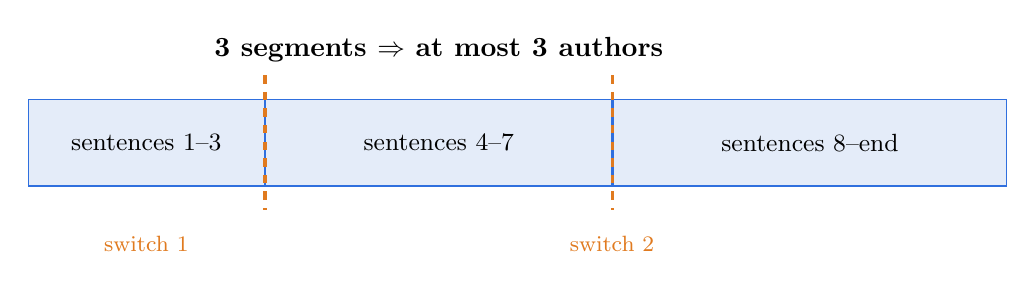
\begin{tikzpicture}[
  seg/.style={draw=accent,fill=soft,minimum height=1.1cm,align=center,font=\small},
  cut/.style={draw=accent2,very thick,dashed}]
\node[seg,minimum width=3cm] (s1) {sentences 1--3};
\node[seg,minimum width=4.4cm,right=0pt of s1] (s2) {sentences 4--7};
\node[seg,minimum width=5cm,right=0pt of s2] (s3) {sentences 8--end};
\draw[cut] ($(s1.north east)+(0,0.3)$) -- ($(s1.south east)+(0,-0.3)$);
\draw[cut] ($(s2.north east)+(0,0.3)$) -- ($(s2.south east)+(0,-0.3)$);
\node[below=0.5cm of s1,font=\footnotesize,text=accent2] {switch 1};
\node[below=0.5cm of s2,font=\footnotesize,text=accent2,xshift=2.2cm] {switch 2};
\node[above=0.35cm of s2,font=\bfseries] {3 segments $\Rightarrow$ at most 3 authors};
\end{tikzpicture}
\bigskip

\raggedright
\begin{itemize}\itemsep0.4em
\item The number of segments gives an \textbf{upper bound} on the number of authors
\item How tight that bound is depends on how accurate the switch detector is
\end{itemize}
\end{frame}

% \begin{frame}{Number of authors: estimating it}
% \begin{columns}[T]
% \begin{column}{0.58\textwidth}
% \textbf{Plan}
% \begin{enumerate}\itemsep0.4em
% \item Use switch detection accuracy to set the maximum number of authors $K_{\max}$ = number of segments
% \item Represent each segment with the same stylometric features (averaged over its sentences)
% \item Train clustering algorithms on the segments (e.g.\ k-means, hierarchical, Gaussian mixture)
% \item Choose $k \le K_{\max}$ with an internal criterion such as silhouette score
% \item Estimated authors $=k$
% \end{enumerate}
% \end{column}
% \begin{column}{0.42\textwidth}
% \begin{block}{Caveats}
% \small
% \begin{itemize}\itemsep0.3em
% \item Missed switches undercount segments, so recall limits the bound
% \item False switches inflate it, which clustering can merge back
% \item On medium/hard data the detector is near chance, so better features come first
% \end{itemize}
% \end{block}
% \end{column}
% \end{columns}
% \end{frame}

\begin{frame}{Summary}
\begin{itemize}\itemsep0.7em
\item Author Switch Detection system: 9 features + hashed tri-gram profile and distance: 11-value pair feature vector
\item The results are baseline F1 (0.435 - 0.456)
\end{itemize}
\vfill
\centering{\Large\color{accent}Thank you. Questions?}
\end{frame}

\end{document}
